\documentclass[12pt,a4paper,notitlepage]{report}
\usepackage[utf8]{inputenc}
\usepackage[spanish]{babel}

\usepackage{afterpage}
\usepackage{enumitem}
\setlist[enumerate]{label*=\arabic*.}
\usepackage{hyperref}
\usepackage{longtable}
\usepackage[outputdir=build]{minted}
\usepackage{csquotes}

\usepackage{graphicx}
\usepackage{xcolor}
\usepackage{xcolor-solarized}
\usepackage[pagecolor=none]{pagecolor}

\usepackage[backend=biber]{biblatex}
\usepackage[acronym]{glossaries}
\usepackage{glossaries-extra}

\usepackage{pmboxdraw}

\usepackage{lipsum}

\makeglossaries
\addbibresource{tex/misc/db_bibliography.bib}
\newglossaryentry{acid}{
  type=\acronymtype,
  name={ACID},
  description={Atomicity Consistency Isolation Durability},
  first={Atomicity Consistency Isolation Durability (ACID)}
}

\newglossaryentry{api}{
  type=\acronymtype,
  name={API},
  description={Application Programming Interface},
  first={Application Programming Interface (API)},
  see=[véase:]{apig}
}

\newglossaryentry{bdd}{
  type=\acronymtype,
  name={BDD},
  description={Behavior-Driven Development},
  first={Behavior-Driven Development (BDD)},
  see=[véase:]{bddg}
}

\newglossaryentry{crud}{
  type=\acronymtype,
  name={CRUD},
  description={Create, Read, Update, Delete},
  first={Create, Read, Update, Delete (CRUD)}
}

\newglossaryentry{dbal}{
  type=\acronymtype,
  name={DBAL},
  description={Database Abastraction Layer},
  first={Database Abstraction Layer (DBAL)},
  see=[véase:]{dbalg}
}

\newglossaryentry{dql}{
  type=\acronymtype,
  name={DQL},
  description={Doctrine Query Language},
  first={Doctrine Query Language (DQL)}
}

\newglossaryentry{dto}{
  type=\acronymtype,
  name={DTO},
  description={Data Transfer Object},
  first={Data Transfer Object (DTO)},
  see=[véase:]{dtog}
}

\newglossaryentry{pfm}{
  type=\acronymtype,
  name={PFM},
  description={Proyecto de Fin de Máster},
  first={Proyecto de Fin de Máster (PFM)}
}

\newglossaryentry{edt}{
  type=\acronymtype,
  name={EDT},
  description={Estructura de Descomposición de Trabajo},
  first={Estructura de Descomposición de Trabajo (EDT)}
}

\newglossaryentry{hateoas}{
  type=\acronymtype,
  name={HATEOAS},
  description={Hypermedia As The Engine Of Application State},
  first={Hypermedia As The Engine Of Application State (HATEOAS)},
  see=[véase:]{hateoasg}
}

\newglossaryentry{html}{
  type=\acronymtype,
  name={HTML},
  description={HyperText Markup Language},
  first={HyperText Markup Language (HTML)}
}

\newglossaryentry{jwt}{
  type=\acronymtype,
  name={JWT},
  description={JSON Web Token},
  first={JSON Web Token (JWT)}
}

\newglossaryentry{kvm}{
  type=\acronymtype,
  name={KVM},
  description={Kernel Virtual Machine},
  first={Kernel Virtual Machine (KVM)},
  see=[véase:]{kvmg}
}

\newglossaryentry{orm}{
  type=\acronymtype,
  name={ORM},
  description={Object Relational Mapping},
  first={Object Relational Mapping (ORM)},
  see=[véase:]{ormg}
}

\newglossaryentry{php}{
  type=\acronymtype,
  name={PHP},
  description={PHP: Hypertext Preprocessor},
  first={PHP: Hypertext Preprocessor (PHP)}
}

\newglossaryentry{mvc}{
  type=\acronymtype,
  name={MVC},
  description={Modelo Vista Controlador},
  first={Modelo Vista Controlador (MVC)}
}

\newglossaryentry{rdbms}{
  type=\acronymtype,
  name={RDBMS},
  description={Relational Database Management System},
  first={Relational Database Management System (RDBMS)}
}

\newglossaryentry{rest}{
  type=\acronymtype,
  name={REST},
  description={Representational State Transfer},
  first={Representational State Transfer (REST)},
  see=[véase:]{restg}
}

\newglossaryentry{sql}{
  type=\acronymtype,
  name={SQL},
  description={Structured Query Language},
  first={Structured Query Language (SQL)}
}

\newglossaryentry{tdd}{
  type=\acronymtype,
  name={TDD},
  description={Test Driven Development},
  first={Test Driven Development (TDD)},
  see=[véase:]{tddg}
}

\newglossaryentry{url}{
  type=\acronymtype,
  name={URL},
  description={Uniform Resource Identifier},
  first={Uniform Resource Identifier (URL)}
}

\newglossaryentry{accidentalComplexity}{
  name=Complejidad Accidental,
  description={
    Se llama así a la complejidad que no está asociada con la búsqueda y
    desarrollo de la solución en sí, sino a la que está asociada al uso de
    herramientas o el desarrollo de las mismas para alcanzar dicha solución
  }
}

\newglossaryentry{apig}{
  name=API,
  description={
    Grupo de procedimientos definidos que facilitan la comunicación entre
    componentes de software
  }
}

\newglossaryentry{bddg}{
  name=Behavior-Driven Development,
  description={
    Se considera una extensión de \gls{tdd} que hace uso de un
    \glslink{lde}{lenguaje de dominio específico} para convertir sentencias
    escritas en lenguaje natural en pruebas ejecutables \cite{bdd_wiki}
  }
}

\newglossaryentry{backend}{
  name=Back End,
  description={
    Capa de lógica y acceso a datos del software
  }
}

\newglossaryentry{cookie}{
  name=Cookie,
  description={
    Pequeño fragmento de datos que las aplicaciones web envían a los usuarios,
    y que generalmente estos últimos almacenan en su navegador, con la finalidad
    de guardar cierta información de estado \textemdash como por ejemplo
    sesiones, opciones de personalización de la aplicación o la lista del
    carro de la compra digital\textemdash. Después esta información se manda
    de vuelta al servidor para que este último adecúe la aplicación al usuario
    que mandó la petición \cite{cookies_wiki}
  }
}

\newglossaryentry{dbalg}{
  name=DBAL,
  description={
    \gls{api} que tiene como objetivo unificar la comunicación entre la
    aplicación y las distintas tecnologías de bases de datos, como pueden ser
    MariaDB, MySQL, SQL Server, etc. La idea es proveer al desarrollador una
    única interfaz que le evite tener que programar una interfaz por
    tecnología de base de datos \cite{dbal_wiki}
  }
}

\newglossaryentry{frontend}{
  name=Front End,
  description={
    Capa de visualización del software
  }
}

\newglossaryentry{hateoasg}{
  name=HATEOAS,
  description={
    Restricción de la arquitectura \gls{rest}, la cual pretende proveer de
    indicaciones al consumidor de la \gls{api} sobre qué pasos se pueden dar en
    ese punto mediante enlaces a las siguientes operaciones disponibles. En un
    contexto de una aplicación de un banco, la respuesta que un cliente
    recibiría al hacer una llamada a una operación de consulta de saldo, podría
    incluir los enlaces a las operaciones de \textit{transferencia},
    \textit{extracción de dinero} o \textit{consultar movimientos}, por ejemplo
    \cite{hateoas_so} \cite{hateoas_wiki}
  }
}

\newglossaryentry{modentrel}{
  name=Modelo entidad-relación,
  description={
    Un modelo entidad-relación o diagrama \\ entidad-relación es una herramienta
    para el modelado de datos que permite representar las entidades relevantes
    de un sistema de información así como sus interrelaciones y propiedades
  }
}

\newglossaryentry{jira}{
  name=Jira,
  description={
    Software de seguimiento de proyectos e incidencias
  }
}

\newglossaryentry{lde}{
  name=Lenguaje de dominio específico,
  description={
    El \textit{LDE} o más conocido como \textit{DSL} \\ \textemdash Domain
    Specific Language\textemdash por sus siglas en inglés, es un lenguaje
    informático especializado en un dominio específico, con el objetivo de
    facilitar la representación de problemas y la resolución de los mismos
    \cite{dsl_wiki}
  }
}

\newglossaryentry{ormg}{
  name=ORM,
  description={
    Esta técnica permite realizar mapeos de objetos y sus atributos a tablas
    relacionales
  }
}

\newglossaryentry{pruebascajanegra}{
  name=Pruebas de caja negra,
  description={
    Las pruebas de caja negra son aquellas que analizan la funcionalidad de una
    aplicación sin tener en cuenta la estructura interna o el funcionamiento de
    dicha funcionalidad \cite{blackbox_wiki}, centrándose en proporcionar a la
    funcionalidad una entrada y comprobando que la salida sea la esperada
  }
}

\newglossaryentry{restg}{
  name=REST,
  description={
    Los servicios web \gls{rest} son una herramienta que facilitan el
    intercambio de información, y el uso de dicha información intercambiada
    entre sistemas informáticos en internet. Dichos servicios hacen uso de una
    serie de operaciones sin estados, que devuelven un resultado al consumidor
    de dicho servicio, generalmente en formato XML, HTML, JSON o cualquier otro
    formato definido
  }
}

\newglossaryentry{semanticweb}{
  name=Web semántica,
  description={
    La web semántica es una extensión de la web que mediante estándares
    propuestos por la W3C, pretenden impulsar formatos de datos comunes, como
    pueden ser el RDFa, JSON-LD o HAL. De esta forma, se intenta impulsar una
    web contextualizada en la que los datos tengan relación entre sí, incluso
    si dichos datos están diseminados por distintos recursos web \cite{semweb}
  }
}

\newglossaryentry{swaggerui}{
  name=Swagger UI,
  description={
    Interfaz de usuario que muestra de forma muy amigable las operaciones de
    una \gls{api}, además de ofrecer la posibilidad de interactuar con dichas
    operaciones en la misma página donde se muestran. Esta documentación se
    genera a partir de una especificación denominada Swagger
  }
}

\newglossaryentry{testsfuncionales}{
  name=Pruebas funcionales,
  description={
    Las pruebas funcionales o \textit{functional testing} se consideran como
    un proceso para asegurar la calidad del software, y también como un
    tipo de pruebas de la modalidad \glslink{pruebascajanegra}{caja negra}.
    Generalmente, este tipo de pruebas se realizan introduciendo una entrada y
    analizando la salida de la funcionalidad en cuestión que se está probando,
    comprobando que todo funciona según las especificaciones de dicha
    funcionalidad \cite{functionalt_wiki}
  }
}

\newglossaryentry{webframework}{
  name=Web Framework,
  description={
    Un \textit{Web Framework} es una abstracción en la que un software que
    provee de una funcionalidad genérica puede ser selectivamente modificada
    adiciones, modificaciones o eliminaciones de código. Estos
    \textit{frameworks} ayudan en el desarrollo de aplicaciones web, incluyendo
    servicios web, recursos web y \gls{api}s web. El objetivo de estas
    herramientas es el de automatizar ciertas tareas y ahorrar tiempo en las
    actividades comunes asociadas al desarrollo web
  }
}

\newglossaryentry{tddg}{
  name=Test Driven Development,
  description={
    El \gls{tdd} es un proceso de desarrollo de software que se basa en la
    repetición de un ciclo de desarrollo muy corto: los requerimientos se
    convierten en casos de pruebas muy específicos, y únicamente está permitido
    programar para hacer que dichos casos de prueba se realicen
    satisfactoriamente
  }
}


\glsaddall

\setcounter{biburllcpenalty}{7000}
\setcounter{biburlucpenalty}{8000}

\begin{document}
  \hypersetup{pageanchor=false}
  \pagenumbering{roman}

  % Heavily based on https://en.wikibooks.org/wiki/LaTeX/Title_Creation. Thank you!
\begin{titlepage}

  \pagecolor{black}\afterpage{\nopagecolor}
  \afterpage{\null\thispagestyle{empty}\newpage}

  \color{white}
  \centering

  
\includegraphics[scale=0.2]{img/logo_upvehu}\par
  
\includegraphics[scale=0.3]{img/logo_gugocreative}\par\vspace{1cm}

  \vspace{3cm}

  {\scshape\Large Proyecto de Fin de Máster \par}

  \vspace{1.5cm}

  {\Huge\bfseries Título del proyecto\par}

  \vfill

  \Large Mikel Alejo Barcina Ribera\par
  {\itshape mabarcina001@ikasle.ehu.eus}

\end{titlepage}


  \setcounter{page}{3}

\pdfbookmark[0]{Dedicatoria}{dedicatory}

\lipsum[1]


  \newpage

  \pdfbookmark[0]{Agradecimientos}{agradecimientos}

\renewcommand{\abstractname}{Agradecimientos}

\begin{abstract}

  \lipsum[1]

\end{abstract}


  \newpage

  \begin{abstract}

  \lipsum[1]

\end{abstract}


  \newpage

  \pagenumbering{Roman}

  \tableofcontents

\newpage

\listoffigures

%\newpage

%\listoftables

  \newpage

  \hypersetup{pageanchor=true}
  \pagenumbering{arabic}

  \chapter{Gestión del proyecto}

\section{Gestión del alcance del proyecto}
La propuesta del proyecto incluye unas indicaciones generales de cómo quiere
la empresa que sea la aplicación, pero son insuficientes para poder realizar
un análisis realista del alcance que va a tener el proyecto.

Además, hay que tener en cuenta que el objetivo de este proyecto es realizar
una aplicación que funcione de forma cohesionada entre los diferentes
departamentos de la empresa, por lo que es muy probable que las
requerimientos cambien a lo largo del desarrollo del proyecto, o se tengan
que modificar.

\subsection{Planificación de la gestión del alcance}
El alcance del proyecto se generará una vez se conozcan, validen y contrasten
todos los requerimientos recogidos. Después, se generará la \gls{edt} una vez
se disponga de la primera versión del alcance, e incluirá todos los aspectos
del \gls{pfm}: planificación, gestión, desarrollo, seguimiento y control y
cierre.

El seguimiento y control del alcance se realizará a lo largo del desarrollo
del proyecto, revisando también los requerimientos, para evaluar si será
necesaria la aplicación de una modificación al alcance y al \gls{edt}. Antes de
hacer efectiva una modificación se tendrá que evaluar y comprobar que la
aplicación de dicha modificación no afecte a la viabilidad del proyecto.
Seguidamente se comprobará el \gls{edt} y se verificará si es necesario también
un cambio en dicha estructura.

\subsection{Planificación de la gestión de requerimientos}
\label{subsec:pgr}
Los trabajadores usan actualmente una aplicación determinada de seguimiento y
control de tiempos, clientes y proyectos. Es por ello que es crucial realizar
entrevistas con los trabajadores de los diferentes departamentos para extraer
de sus respuestas aquellas cosas que les gustan, las que no, y las que
mejorarían, además de su experiencia en general usando dicha aplicación. Al
procesar estas respuestas se podrán obtener los requerimientos del producto
a desarrollar y, finalmente, su validación consistirá en exponer dichos
requerimientos ante los interesados del proyecto, dando su visto bueno o no
a aquellos puntos con los que estén de acuerdo.

El seguimiento y control de los requerimientos se realizará a lo largo del
desarrollo del proyecto, cuando los diferentes interesados de la aplicación
contrasten que los requerimientos indicados y las que finalmente han sido
implementadas coinciden.

En caso de que los requerimientos tengan que sufrir algún cambio, se
evaluará si el nuevo requerimiento, o la modificación de uno ya existente,
es viable y se puede llevar a cabo. Se podrá modificar la prioridad e
importancia de los diferentes requerimientos, e incluso descartar unos
requerimientos por otros. En caso de que los cambios en los requerimientos
supongan un cambio drástico en el proyecto, se realizará una reunión con
los interesados del proyecto para ratificar dicho cambio.

\subsection{Recopilación de requerimientos}
\label{subsec:rdr}
Tras realizar el proceso descrito en \ref{subsec:pgr}, se validaron los
siguientes requerimientos que deberá tener la aplicación, ordenados por 
importancia:

\begin{enumerate}
 \item Desarrollar un \gls{backend} en forma de \gls{api} \gls{rest} que
 permita intercambiar datos con un \gls{frontend}

 \item El \gls{backend} ha de proporcionar control de acceso para restringir el
 contenido visible \textemdash ya sea restringiendo el acceso a recursos
 completos o limitando la información mostrada en recursos específicos
 \textemdash dependiendo de una serie de roles.

 \item Los proyectos de la aplicación deberán tener una estructura común, y
 los gestores deberán tener la opción de modificar dicha estructura según
 las necesidades específicas de cada proyecto.

 \item La aplicación permitirá crear informes que recopilen datos por proyecto,
 departamento y por trabajador.

 \item La aplicación permitirá crear listas de favoritos, plantillas, o
 reordenar las tareas por usuario para facilitar la imputación de horas.

 \item La aplicación permitirá cerrar y reabrir los proyectos.

 \item La aplicación permitirá enviar recordatorios a aquellos usuarios que
 se les haya olvidado imputar horas.

 \item La aplicación permitirá a los gestores de proyectos imputar horas a
 terceras personas, por ejemplo en el caso de que haya un trabajador por cuenta
 propia contratado.

 \item La aplicación tendrá una integración con \gls{jira}

 \item La aplicación permitirá crear procesos a los gestores para facilitar
 la gestión.

 \item La aplicación permitirá visualizar de forma sencilla qué personas
 están de vacaciones.

 \item Todos los proyectos tendrán que compartir los mismos colores en las
 categorías comunes.

 \item Una aplicación de escritorio que facilite la imputación de horas
 y, que entre las funcionalidades estándar de la aplicación, tenga una que
 ayude a realizar el seguimiento de la tarea que se está realizando en
 ese momento mediante un botón \textit{play / stop}.

 \item La interfaz ha de ser rápida y sencilla de usar para imputar horas de
 tareas individuales y un grupo de tareas.

 \item La interfaz ha de mostrar a cada usuario cuántas horas ha imputado
 a lo largo de la semana y cuántas le restan por imputar para completar sus
 horas semanales.

 \item La interfaz ha de mostrar sugerencias para las imputaciones: que analice
 las últimas imputaciones para recomendar y ayudar a imputar cuando se trabaja
 en las mismas tareas o en los mismos proyectos.

 \item La interfaz ha de permitir a cada usuario limitar su vista de horas a la
 jornada laboral que realiza, ahorrando así el tener que deslizarse hasta la
 hora de inicio y hora de finalización de la jornada.

 \item La interfaz ha de permitir a cada usuario configurar la vista de las
 imputaciones: diaria, semanal y mensual.
\end{enumerate}

\subsection{Alcance}
Los requerimientos recogidos abarcan tanto el diseño, desarrollo e
implementación tanto del \gls{backend} como del \gls{frontend} de la
aplicación. No obstante, debido al límite de recursos del que se dispone
para la realización del \gls{pfm}, he decidido junto con la empresa el
centrarme en el desarrollo de un \gls{backend} seguro, robusto y fiable
mientras que otra persona realizará el \gls{frontend}. Esta decisión se ha
tomado, a parte de por el motivo del límite de recursos, para evitar que
se acabe el \gls{pfm} con un producto a medias y sin finalizar. Por lo tanto,
los requerimientos que quedan dentro del alcance de este \gls{pfm} son: los
requerimientos del 1 al 8 del apartado \ref{subsec:rdr}, y los dos siguientes,
el 9 y el 10, se consideran funcionalidades opcionales a desarrollar si los
recursos restantes lo permiten.

\subsection{EDT}
\begin{verbatim}
Clepsydra
├ Gestión
│ └ Planificación
│   ├ Alcance
│   │ ├ Gestión del alcance
│   │ ├ Gestión de requerimientos
│   │ ├ Requerimientos
│   │ ├ Alcance
│   │ ├ EDT
│   │ ├ Gestión de la validación del alcance
│   │ └ Gestión del seguimiento y control del alcance
│   ├ Tiempo
│   │ ├ Gestión del tiempo
│   │ ├ Definición de actividades
│   │ ├ Estimación de la duración de las actividades
│   │ └ Gestión del seguimiento y control de las actividades
│   ├ Calidad
│   │ ├ Gestión de la calidad
│   │ ├ Calidad mínima y calidad añadida
│   │ └ Gestión del seguimiento y control de la calidad
│   ├ Riesgos
│   │ ├ Gestión de riesgos
│   │ ├ Riesgos
│   │ └ Planes de contingencia
│   ├ Seguimiento y control
│   │ ├ Seguimiento y control del alcance
│   │ ├ Seguimiento y control del tiempo
│   │ ├ Seguimiento y control de la calidad
│   │ └ Seguimiento y control de los riesgos
│   └ Cierre
│     ├ Gestión del cierre
│     ├ Presentación del PFM
│     └ Cierre
├ Diseño
│ ├ Diseño de la base de datos
│ ├ Diseño de los casos de uso
│ └ Diseño y documentación de la API
└ Desarrollo
  ├ Formación
  ├ Implementación
  ├ Corrección de errores
  └ Testing
\end{verbatim}

\subsection{Validación del alcance}
La validación del alcance se hará junto con los requerimientos del proyecto,
en una reunión con los interesados del proyecto. En el caso de que se propongan
alteraciones se tomarán en consideración y se realizarán las modificaciones
oportunas acorde con lo expuesto.

En caso de que sea necesario modificar el alcance a lo largo del ciclo de
vida del proyecto, se tendrán que validar dichos cambios con los diferentes
interesados.

\subsection{Seguimiento y control del alcance}
El seguimiento del alcance se realizará periódicamente, cada Lunes de cada
semana, desde la fecha de inicio del desarrollo de la aplicación, comprobando
qué requerimientos se han cumplido, cuales faltan por cumplir, y cuales hay
que descartar en el caso de que no se dispongan de los suficientes recursos
para dedicar a dichos requerimientos.

\section{Gestión del tiempo}
\subsection{Planificación de la gestión del tiempo}
Una vez se hayan conocido todos los requerimientos y se haya definido el
alcance del proyecto, se procederá a realizar la primera estimación general
del mismo. Para la parte de la estimación del desarrollo del producto, se
pedirá opinión y quizás alguna directriz a algunos profesionales de la empresa,
los cuales ya han trabajado en productos similares. De esta forma se podrá
realizar una estimación más precisa. Se definirán las actividades con la
máxima precisión posible, intentando minimizar el tener que definir más tareas
a lo largo del proyecto.

En el caso en el que sea necesario modificar la lista de actividades, se
añadirán, modificarán o quitarán siempre teniendo en cuenta el alcance, los
requerimientos y los recursos disponibles para el proyecto, de forma que
no se ponga en peligro la viabilidad del mismo.


\subsection{Definición de actividades}

\subsection{Secuencia de actividades}

\subsection{Estimación de la duración de las actividades}

\subsection{Seguimiento y control}
La unidad de tiempo mínima que se utilizará para realizar el seguimiento y
control de cada actividad será de 15 minutos. Dichas actividades y el tiempo
invertido en cada una de ellas será recogido en una tabla donde quede reflejada
toda la información pertinente.

\section{Gestión de calidad}
\subsection{Planificación de la gestión de la calidad}
La calidad del producto se definirá mediante dos grupos: la calidad
mínima y la calidad extra. Los elementos de calidad mínima serán
aquellos que son indispensables para poder realizar un cierre
satisfactorio y exitoso del proyecto. Por contra, los elementos que se
agrupen dentro de la calidad extra, serán aquellos a los que se les
dedicarán recursos siempre y cuando la calidad mínima en el producto
haya sido conseguida.

En el caso de que se propongan nuevas ideas, características o
requerimientos para el producto final, se tendrá que hacer una
evaluación de dichas características para decidir en qué grupo habrá de
clasificarla.

Por último, si uno de los elementos considerados de calidad mínima no
puede ser completado o desarrollado, se estudiará la posibilidad de
moverlo al grupo de elementos de calidad extra, siempre teniendo en
cuenta la opinión de los interesados del proyecto.

\subsection{Calidad mínima}
\label{sec:min:qual}
Los elementos que se incluirán en el producto, y que se consideran que
son indispensables para el mismo, son los elementos del 1 al 10, especificados 
en la sección de requerimientos \ref{enum:req:lis}.

Además, se hará hincapié en las pruebas del producto o \textit testing \textit,
con el objetivo de que el producto pueda ser considerado estable y robusto, y
que sobre todo asista en el desarrollo a la hora de modificar el susodicho
producto, indicando qué partes funcionan y cuales no a la hora de introducir
los cambios.

\subsection{Calidad añadida}
\label{sec:add:qual}
Los elementos de calidad añadida para el producto son los elementos 11,
12 y 13 especificados en la sección de requerimientos \ref{enum:req:lis}.

\subsection{Seguimiento y control de la calidad}
El seguimiento y control de la calidad se irá haciendo en conjunción con
el seguimiento y control de los requerimientos \ref{subsec:syc:scope},
el alcance \ref{subsec:syc:scope} y las actividades
\ref{subsec:syc:timeManagement}, y dependiendo del estado general del
conjunto del proyecto se tomarán las decisiones oportunas.

\section{Gestión de riesgos}
\subsection{Planificación de la gestión de riesgos}
Los riesgos se identificarán y recogerán en una lista, y posteriormente
se elaborarán planes de contingencia para lidiar con los problemas que
los riesgos puedan plantear en un futuro.

\subsection{Identificación de riesgos}
\label{section:risks}
\begin{itemize}
    \item No cumplir con la calidad mínima especificada.
\end{itemize}
A pesar de que se tiene noción sobre las tecnologías que se verán
involucradas en el producto, nunca se ha realizado ningún desarrollo
similar en un entorno real con proyección a comercializar el producto.
Es por ello que puede resultar que las estimaciones realizadas sean
insuficientes y que no se satisfaga el alcance definido. Este riesgo
por lo tanto se considera un riesgo alto.

\begin{itemize}
    \item No tener un producto mínimo que sea funcional cuando el otro
        integrante comience a desarrollar su parte.
\end{itemize}
Relacionado con el riesgo anterior, puede darse la situación en la que
el producto no sea mínimamente funcional cuando el otro integrante
comience su desarrollo. Este riesgo se clasifica como de nivel medio.

\subsection{Planes de contingencia}
\label{section:continplans}
\begin{itemize}
    \item No cumplir con la calidad mínima especificada.
\end{itemize}
A la hora de desarrollar, se priorizarán aquellas funcionalidades y
especificaciones que tengan que ver con los requerimientos, y si aún y
todo el tiempo para cumplir con la calidad mínima empieza a escasear,
se centrará el desarrollo en dichas funcionalidades.

Si el problema es debido a la falta de recursos, se valorará la
aceptación del producto desarrollado con los interesados del producto.
En caso afirmativo, se dará por concluido el mismo y se aceptará el
cierre de la parte de desarrollo del proyecto. En caso negativo, el
proyecto se cerrará y se marcará como inacabado.

\begin{itemize}
    \item No tener un producto mínimo que sea funcional cuando el otro
        integrante comience a desarrollar su parte.
\end{itemize}
En este caso se abandonará cualquier otro trabajo para centrarse en
proporcionar al otro integrante un producto funcional con el que pueda
probar su desarrollo.

\subsection{Seguimiento y control de la calidad}
El seguimiento y control de los riesgos se realizará a lo largo del
proyecto, y se recogerán las incidencias, si hubiere, en un apartado
que indique la aplicación de los planes de contingencia propuestos y la
forma en la que se han llevado a cabo.


\chapter{Diseño y desarrollo del producto}
\section{Contexto}

\subsection{Contexto de la empresa}
\label{context:company}

GuGo Creative S.L. es una pequeña empresa localizada en Donostia, la
cual centra su actividad en el diseño y desarrollo de soluciones web
y también en el diseño y desarrollo de aplicaciones móviles.

\subsection{Contexto del proyecto propuesto}
La empresa utilizaba una aplicación de seguimiento y control de tiempos,
que permitía dar de alta clientes, proyectos y tareas, y que recogía
las imputaciones de tiempo que los trabajadores dedicaban a cada
proyecto. El objetivo era generar un informe para después exportarlo,
y mediante un programa externo obtener las rentabilidades de los
proyectos y los clientes.

Según se me informó, dicha aplicación la escogieron después de hacer un
estudio de las diferentes alternativas existentes, pero aún y todo, no
suplía todas las necesidades específicas de la empresa y además, tenía
funcionalidades que no se utilizaban en absoluto.

Por todo ello, se propuso realizar un desarrollo propio, el cual
supliera las necesidades que tenía la empresa, y fuera suficientemente
extensible o modificable para poder comercializar el producto para otras
empresas.


\section{Tecnologías involucradas}
\subsection{Asunciones previas}
Como se ha indicado en la sección del contexto de la empresa
\ref{context:company}, su especialidad son los desarrollos web y de
aplicaciones móviles. Es por ello que desde el principio se habló de que el
desarrollo de la \gls{api}, sería un desarrollo web.

\subsubsection{Tecnología propuesta}
Debido a que la empresa cuenta con trabajadores que ya realizaron proyectos con
una tecnología específica, se me pidió que usara la susodicha tecnología para
así facilitar la modificación, adaptación o corrección de errores una vez el
proyecto estuviera finalizado. La tecnología propuesta, por lo tanto, fue
Symfony.

\subsection{Frameworks utilizados en la aplicación}

\subsubsection{Symfony}
Symfony es un \glslink{webframework}{framework} escrito en \gls{php} y
organizado en \textit{bundles} o paquetes que permite realizar desarrollos web
disminuyendo la \gls{accidentalComplexity}. De hecho, una de las
características de Symfony es que absolutamente todo se organiza en paquetes.
Incluso el propio \glslink{webframework}{framework}, es un paquete. Otro de los
puntos fuertes de Symfony es que gracias a cómo ha sido desarrollado, fuerza a
programar siguiendo buenas prácticas y patrones conocidos, que hacen que la
calidad del código aumente.

\subsubsection{API Platform}
\label{tech:apiplat}
API Platform es a su vez otro \glslink{webframework}{framework} que está
diseñado especialmente para funcionar sobre Symfony, y que facilita la creación
de \gls{api}s. Una de sus características más llamativas es que una vez
definidas las entidades del dominio en clases \gls{php}, API Platform genera
automáticamente operaciones \gls{crud}. Otras de las funcionalidades destacables
que tiene, son entre otras:

 \begin{itemize}
    \item Soporte para diferentes formatos: XML, JSON, CSV y YAML.
    \item Soporte para la \glslink{semanticweb}{web semántica}: JSON-LD y HAL.
    \item Soporte para \gls{api}s \gls{hateoas}.
    \item Generación automática de documentación para las operaciones de la
        \gls{api} mediante \gls{swaggerui}.
    \item Paginación de resultados.
    \item Filtros de resultados.
 \end{itemize}

\subsection{Librerías destacables utilizadas en la aplicación}
Las dependencias de librerías externas en \gls{php} se suelen gestionar con
\textit{Composer}: este programa utiliza un fichero JSON que va llevando cuenta
de las dependencias requeridas y en qué versión se instalaron, de forma que los
proyectos no necesitan incluir dichas librerías cuando se despliegan o cuando
los diferentes miembros que contribuyen en él hacen acopio del código fuente.
Con un simple comando, \textit{Composer} leerá las dependencias requeridas y
las descargará desde el repositorio localizado en \url{https://packagist.org/}.
El formato en el que se recogen las librerías sigue el patrón
\textit{vendor/package}, y es el que utilizaré para describir algunas de las
librerías más interesantes utilizadas en el proyecto.

\subsubsection{api-platform/core}
El núcleo de API Platform. Esta librería es la que facilita las funcionalidades
indicadas en la sección de \glslink{webframework}{frameworks} \ref{tech:apiplat}
.

\subsubsection{symfony/http-foundation}
Define una capa orientada a objetos para la especificación HTTP
\cite{symfony_httpfound}, la cual tiene como finalidad englobar las variables
y funciones que \gls{php} utiliza para gestionar y manipular las peticiones
recibidas y las respuestas generadas\cite{symfony_httpfound_two}. Por ejemplo,
en el siguiente bloque de código, se muestra cómo las variables globales
\textemdash como \textit{\$\_GET} o \textit{\$\_POST}\textemdash que en un
principio habría que gestionar individualmente, se agrupan en cambio en un único
objeto de tipo \textit{Request} mucho más manejable.

\begin{minted}[linenos=true]{php}
<?php

use Symfony\Component\HttpFoundation\Request;

$request = Request::createFromGlobals();

$request = new Request(
    $_GET,
    $_POST,
    array(),
    $_COOKIE,
    $_FILES,
    $_SERVER
);
\end{minted}

La librería también permite acceder a la sesión, a las cabeceras enviadas,
enviar una respuesta, establecer \glslink{cookie}{cookies}, redireccionar
al usuario y múltiples funcionalidades más.

\subsubsection{symfony/http-kernel}
Esta librería se encarga de transformar la petición del usuario recibida en
una respuesta. Para ello, se sirve de el sistema de eventos que tienen
implementado \textemdash \textit{symfony/event-dispatcher}\textemdash el cual
va disparando varios eventos en cada fase de un proceso que se ilustra en la
siguiente ilustración:

\begin{figure}[h]
    \center
    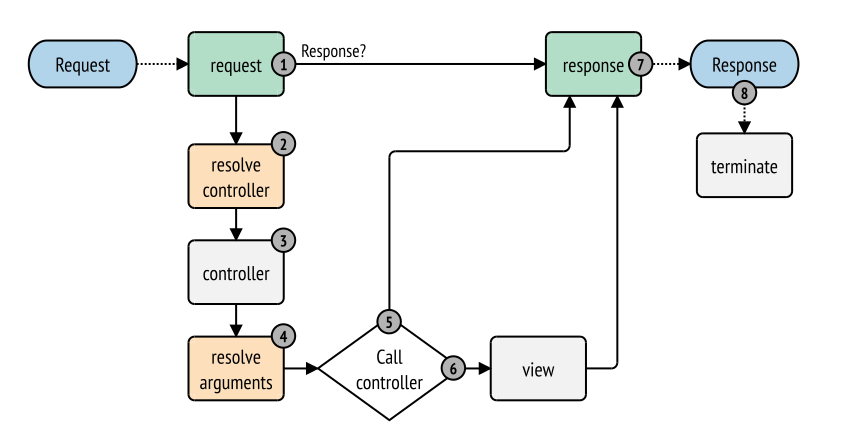
\includegraphics[scale=0.3]{img/http-workflow}
    \caption{Diagrama del proceso de transformación de una petición a una
        respuesta. Fuente:
        \url{https://symfony.com/doc/current/components/http_kernel.html}}
\end{figure}

Cada número representa un paso del proceso, y algunos de estos pasos dispararán
eventos. Al igual que existen eventos, también existen suscriptores a dichos
eventos, que básicamente esperan a que un evento de un tipo determinado se
dispare para realizar una serie de acciones.

\begin{enumerate}
    \item El evento \textit{kernel.request} tiene como objetivo añadir más
        información a la petición \textemdash por ejemplo después de determinar
        en qué idioma debería de darse la respuesta\textemdash, inicializar
        partes del \glslink{webframework}{framework} o crear una respuesta
        inmediatamente y finalizar el proceso: como por ejemplo cuando el
        usuario no tiene la autorización pertinente.
    \item El siguiente paso es averiguar qué controlador ha de llamarse para
        que se ejecute la lógica de negocio acorde a esa respuesta. Esto se
        determina gracias a la información que se extrae de la petición, y a la
        que el programador proporciona al \glslink{webframework}{framework} en
        forma de ciertas directrices como puede ser emparejar una ruta con
        un controlador. Ejemplo: \textit{\"Cuando una petición se realice a la
        ruta /hello/world, se ejecutará la función HelloWorld() del controlador
        HelloWorldController"}.
    \item El evento \textit{kernel.controller} tiene como objetivo preparar la
        ejecución del controlador, ya sea inicializando ciertas partes del
        \glslink{webframework}{framework} o incluso permitiendo que un
        suscriptor cambie el controlador que se va a ejecutar.
    \item En este punto se determinan los argumentos y los valores que han de
        pasarse al controlador. Las formas más comunes de determinarlo suelen
        ser mediante un identificador en la ruta\\ \textemdash
        \textit{/hello/world/argumento1/argumento2}\textemdash, la indicación
        que el programador da para obtener el argumento y finalmente pasando
        directamente la petición al controlador, donde el programador la
        procesará y extraerá los argumentos que le interesen.
    \item Aquí se llama al controlador y se aplica la lógica de negocio
        pertinente según lo que el programador haya programado. En el caso de
        que el controlador devuelva una respuesta, directamente se salta al
        último paso. En caso contrario, se realiza un paso más.
    \item El evento \textit{kernel.view} transforma un resultado de un
        controlador en una respuesta. Aquí es donde suele entrar en juego la
        capa de visualización. Por ejemplo: el controlador devuelve una serie
        de valores que después se insertan en la página correspondiente que
        haya que devolver al usuario, como puede ser el nombre de usuario del
        usuario que realizó la petición.
    \item Finalmente se dispara el evento \textit{kernel.response}, que permite
        a los distintos suscriptores modificar la respuesta antes de que sea
        enviada al usuario.
\end{enumerate}

\subsubsection{symfony/framework-bundle}
La librería encargada de recoger toda la configuración de los diferentes
recursos y elementos que componen el \glslink{webframework}{framework}: las
sesiones, los formularios, validación, enrutamiento\cite{symfony_frambun},
gestión de la capa de visualización, traducciones, cache...

\subsubsection{symfony/security-bundle}
Librería encargada de proporcionar control de acceso a los diferentes recursos
que componen la aplicación. La configuración se realiza mediante parámetros y
patrones de rutas.

\subsubsection{doctrine/orm}
Esta librería provee de \gls{orm} y \gls{dbal} para \gls{php}. Para la
escritura de consultas se utiliza la sintaxis \gls{dql}. He aquí un ejemplo
de una consulta utilizando \gls{dql} y el \textit{Query Builder} de Doctrine:

\begin{minted}[linenos=true]{php}
<?php

$queryBuilder->select('h')
             ->from('house', 'h')
             ->where('h.stories > 2')
             ->orderBy('h.stories', 'ASC');

\end{minted}

\subsubsection{doctrine/annotations}
Esta librería permite realizar anotaciones en las entidades del dominio para
ayudar después a mapear cada atributo y entidad con su tabla y columnas
correspondientes en la base de datos. Un ejemplo de una entidad mapeada podría
ser el siguiente:

\begin{minted}[linenos=true]{php}
<?php

use Doctrine\ORM\Mapping as ORM;

/**
 * @ORM\Entity
 */
class House
{
    /**
     * @ORM\Id()
     * @ORM\GeneratedValue()
     * @ORM\Column(type="integer")
     */
    private $id;

    /**
     * @ORM\Column(type="string", length=255)
     */
    private $name;

    /**
     * @ORM\Column(type="integer")
     */
    private $stories;
}
\end{minted}

\subsubsection{symfony/validator}
Esta librería facilita la validación de los diferentes atributos de las
entidades. La forma de especificación de las restricciones a las cuales están
sujetas, es mediante anotaciones. Así que continuando con el ejemplo anterior:

\begin{minted}[linenos=true]{php}
<?php

use Doctrine\ORM\Mapping as ORM;
use Symfony\Component\Validator\Constraints as Assert;

/**
 * @ORM\Entity
 */
class House
{
    /**
     * @ORM\Id()
     * @ORM\GeneratedValue()
     * @ORM\Column(type="integer")
     */
    private $id;

    /**
     * @ORM\Column(type="string", length=255)
     *
     * @Assert\NotBlank()
     * @Assert\Length(min = 1, max = 255)
     */
    private $name;

    /**
     * @ORM\Column(type="integer")
     *
     * @Assert\GreaterThanOrEqual(0)
     */
    private $stories;
}
\end{minted}

En este simple ejemplo se ha hecho que el atributo \textit{``name''} tenga que
tener una longitud comprendida entre 1 y 255 caracteres, y que el atributo
\textit{``stories''} deba ser mayor o igual que 0. Al quedar las restricciones
plasmadas en la propia entidad, éstas se comprueban para cualquier acceso a
dicha entidad. Por ejemplo, la entidad que se ha usado de ejemplo podría
modificarse mediante un formulario web o una petición a una \gls{api}, pero las
restricciones serán las mismas se modifique de una u otra forma. Huelga decir
que si se requiriese lo contrario, se podría hacer de forma que en el
formulario web se apliquen ciertas restricciones mientras que las llamadas a la
\gls{api} podrían tener restricciones distintas.

\subsubsection{symfony/serializer}
El serializador es un componente que se utiliza para transformar objetos en
formatos específicos, como pueden ser: JSON, XML,
YAML\cite{symfony_serializer}... En el siguiente diagrama se ilustra el
proceso:

\begin{figure}[h]
    \center
    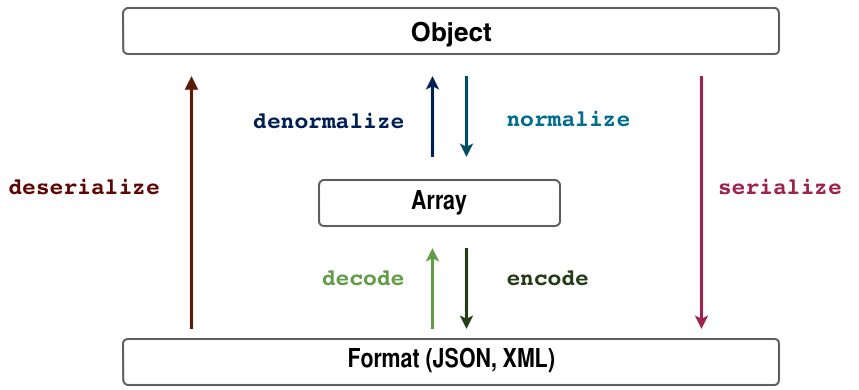
\includegraphics[scale=0.3]{img/serializer_workflow}
    \caption{Diagrama del proceso de serialización de un objeto
      Fuente: \url{https://symfony.com/doc/current/components/serializer.html}}
\end{figure}

Además, mediante el uso de anotaciones, se pueden crear grupos de
serialización, de forma que dependiendo de la petición recibida se pueden
serializar distintos atributos. En el siguiente ejemplo se crean tres grupos,
\textit{private}, \textit{public} y \textit{edit}:

\begin{minted}[linenos=true]{php}
<?php

use Doctrine\ORM\Mapping as ORM;
use Symfony\Component\Serializer\Annotation\Groups;
use Symfony\Component\Validator\Constraints as Assert;

/**
 * @ORM\Entity
 */
class House
{
    /**
     * @ORM\Id()
     * @ORM\GeneratedValue()
     * @ORM\Column(type="integer")
     *
     * @Groups({"private"})
     */
    private $id;

    /**
     * @ORM\Column(type="string", length=255)
     *
     * @Assert\NotBlank()
     * @Assert\Length(min = 1, max = 255)
     *
     * @Groups({"public", "edit"})
     */
    private $name;

    /**
     * @ORM\Column(type="integer")
     *
     * @Assert\GreaterThanOrEqual(0)
     *
     * @Groups({"public"})
     */
    private $stories;
}
\end{minted}

Habiendo etiquetado cada atributo en uno o más grupos de serialización, esto
después puede utilizarse para gestionar de forma dinámica la entidad
dependiendo de las peticiones. Por ejemplo, cuando se hiciera únicamente una
operación de lectura por parte de un cliente sin privilegios, la entidad podría
ser serializada con el grupo \textit{public}, dejando así el atributo
\textit{id} fuera de la respuesta a dar. Lo mismo aplica para los grupos
\textit{edit} que podría utilizarse para limitar las modificaciones a un
atributo en concreto, o el grupo \textit{private} si la casa está siendo
gestionada por un administrador. Los grupos de los nombres en este caso son
esos, pero pueden llamarse como se quiera.

\subsubsection{behat/behat}
Un \glslink{webframework}{framework} \gls{bdd} que permite realizar
\glslink{testsfuncionales}{pruebas funcionales} mediante una sintaxis denominada
\textit{Gherkin}, que facilita la redacción y lectura de las pruebas.
Dichas pruebas se organizan en funcionalidades, escenarios y pasos que después
el \glslink{webframework}{framework} se encarga de ejecutar. Un ejemplo de una
prueba funcional con esta librería podría ser el siguiente:

\begin{minted}[linenos=true]{gherkin}
Feature: House management
  In order to manage houses
  As a house owner
  I need to be able to add a house, modify its parameters or remove it

  Scenario: Modify a house
    Given there exists a house named "My fancy house"
    And I am the owner of it
    When I modify its name to "My beautiful house"
    Then its new name should be "My beautiful house"
\end{minted}

Esta definición de la prueba funcional en \textit{Gherkin} después se mapea a
una clase \gls{php} que interpreta y ejecuta lo que en cada paso debe de
comprobarse:

\begin{minted}[linenos=true]{php}
<?php

class FeatureContext
{
    /**
     * @Given there exists a house named :house
     */
    public function thereExistsHouseNamed($house)
    {
      if(!exists_house($house)) {
        throw new Exception(
          'The house ' . $house . ' doesn't exist'
        );
      }
    }

    /**
     * @Given I am the owner of it
     */
    public function iAmTheOwnerOfTheHouse()
    {
      /** Do stuff */
    }

    /**
     * @When I modify its name to :newName
     */
    public function iModifyItsNameTo($newName)
    {
      /** Do stuff */
    }

    /**
     * @Then its new name should be :expectedName
     */
    public function theNewNameShouldBe($expectedName)
    {
      /** Do stuff */
    }
}
\end{minted}
Este ejemplo se ha simplificado para facilitar la asimilación del concepto
detrás de \textit{Behat}. Una vez hechos los mapeos correctamente
\textit{Behat} se encargará de ejecutar las funciones, y en caso de que no
produzcan ningún error los pasos correspondientes se considerarán como
correctos.

\subsubsection{justinrainbow/json-schema}
Librería utilizada para validar objetos JSON con \textit{JSON Schema}. Por
ejemplo, imaginemos que al realizar una petición al servidor para
obtener información sobre una entidad \textit{House}, dicho servidor devuelve
lo siguiente:
\begin{minted}[linenos=true]{json}
{
  "id": 1,
  "name": "My beautiful house",
  "stories": 2
}
\end{minted}
A la hora de realizar las pruebas de la aplicación, la información que devuelva
el servidor puede ser variada, a pesar de que el entorno de pruebas cargue una
serie de casas predefinidas. En vez de validar que el JSON que devuelve el
servidor es exactamente igual a las diferentes casas que existen en la base de
datos \textemdash porque recordemos que en vez de devolver un único objeto
\textit{House}, el servidor podría devolver un \textit{array} de ellos
\textemdash, se puede comprobar que el objeto JSON devuelto es válido acorde a
un esquema. Por ejemplo:

\begin{minted}[linenos=true]{json}
{
  "type": "object",
  "properties": {
    "id": {"type": "integer"},
    "name": {
      "type": "string",
      "pattern": "^[a-zA-Z0-9]+$"
    },
    "stories": {
      "type": "integer",
      "minimum": 0
    }
  },
  "required": ["id", "name"]
}
\end{minted}
Este esquema, que ha obviado algunos elementos para simplificar el ejemplo,
podría utilizarse para validar las diferentes respuestas que puede dar el
servidor con respecto a diferentes casas. Esto puede resultar muy interesante
para reducir el tamaño de las pruebas y concentrar en un único esquema las
condiciones del objeto JSON que el servidor debería de enviar.

\subsubsection{lexik/jwt-authentication-bundle}
Esta librería provee de una implementación de los \gls{jwt}: Esta tecnología
es un estándar abierto\footnote{\url{https://tools.ietf.org/html/rfc7519}} que
define una forma compacta y autocontenida \textemdash debido a que el token
tiene toda la información del usuario y no es necesario volver a consultar a la
base de datos \textemdash de intercambiar
información entre dos entidades mediante un objeto JSON. Además, la información
puede ser verificada debido a que se firma digitalmente bien utilizando un
secreto, bien utilizando claves públicas y privadas. \cite{jwt_explanation}

Como se ha comentado anteriormente, \gls{jwt} tiene una naturaleza compacta y
autocontenida. Esto es realmente útil, por ejemplo, en arquitecturas \gls{rest}
donde no hay estados: debido a que cada llamada a una \gls{api} \gls{rest} debe
de contener toda la información necesaria para que el servidor pueda procesarla
correctamente, los tokens \gls{jwt} son extremadamente útiles para transmitir,
por ejemplo, la información respecto al usuario que está realizando dicha
llamada. De esta forma el servidor puede extraer todos los datos del token para
comprobarlos y autorizar o no el procesamiento de la petición realizada. He
aquí un diagrama explicando el proceso de inicio de sesión:

\begin{figure}[h]
    \center
    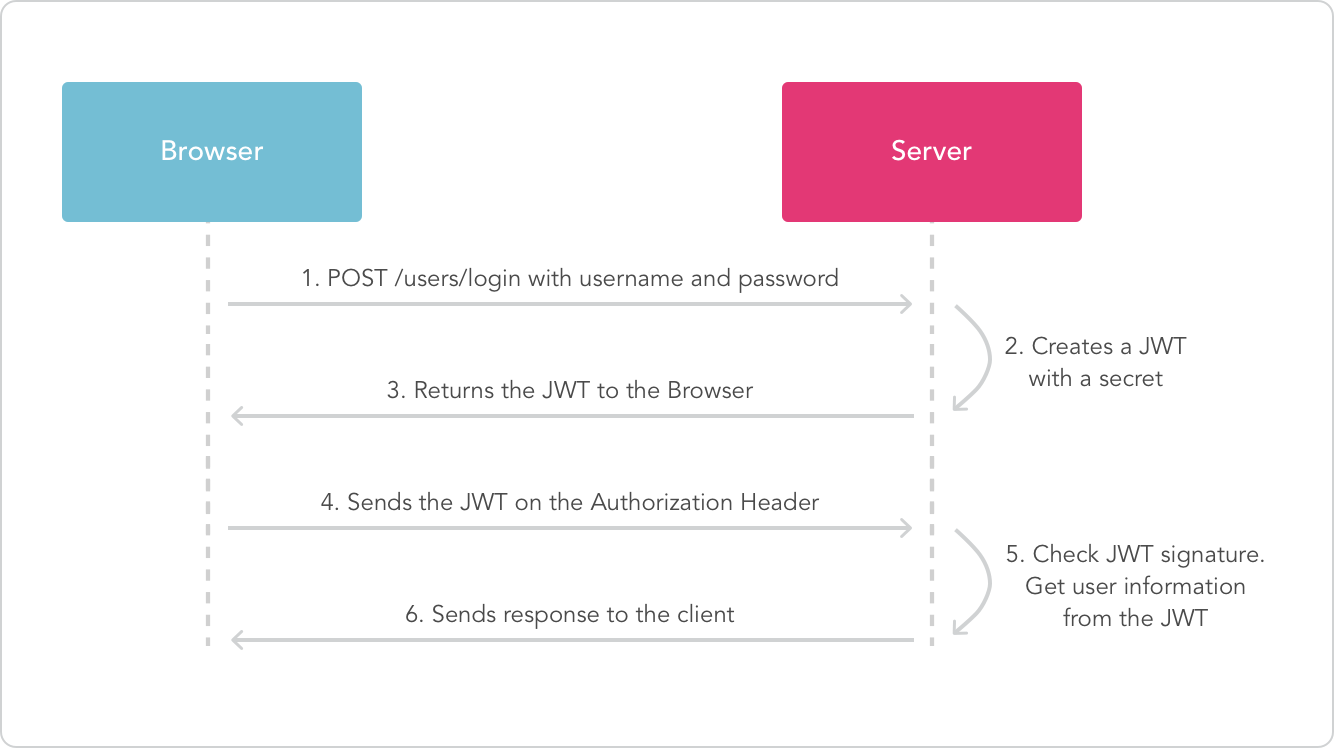
\includegraphics[scale=0.3]{img/jwt-diagram}
    \caption{Diagrama del proceso de inicio de sesión mediante un token
      \textit{JWT}. Fuente:
        \url{https://jwt.io/introduction/}}
\end{figure}

Tal y como se ve en el diagrama, el token \gls{jwt} se envía adjuntado en cada
petición, en una de las cabeceras de la misma: la cabecera
\textit{Authorization}.

\subsubsection{api-platform/api-pack}
Este es un metapaquete el cual agrupa otras librerías que dan la funcionalidad
necesaria para incorporar API Platform en una instalación estándar de Symfony.
Entre otras librerías, incluye \textit{api-platform/core}, que es la librería
que al fin y al cabo provee de las funcionalidades indicadas en la sección de
\glslink{webframework}{frameworks} \ref{tech:apiplat}.


\section{Clepsydra, la aplicación}
\subsection{Arquitectura de la aplicación}
\subsubsection{Servidor}
El servidor donde la aplicación iba a ser probada para su funcionamiento era
una máquina virtual GNU\\Linux que iba sobre una capa de
virtualización \gls{kvm}. Básicamente la empresa ya tenía \gls{kvm} montado y
simplemente tuve que configurar dicho servidor, adhiriéndome a los parámetros
que el informático de sistemas me facilitó.

\subsubsection{Sistema operativo}
El sistema operativo que escogí para montar el servidor fue Debian. El motivo
es que he utilizado mucho la susodicha distribución, y por lo tanto pensé que
sería mucho más fácil configurar una máquina utilizando una tecnología que ya
conocía. Debido a que en la empresa estaban de acuerdo con ello, fue finalmente
la que utilicé.

La distribución se clasifica principalmente en tres ramas: \textit{stable},
\textit{testing} y \textit{unstable}, y debido a que quería ahorrarme
quebraderos de cabeza en el futuro escogí la rama estable de la distribución.

No obstante, debido a su naturaleza estable, algunos de los paquetes que
requería \textemdash principalmente \gls{php} \textemdash no estaban en la
versión que ciertas librerías de la aplicación requerían, por lo que realicé
un pequeño ajuste con lo que se denomina \textit{apt-pinning}.

\textit{apt-pinning} se realiza cuando se precisa obtener versiones de
paquetes, o paquetes enteros, que no están en la rama de la distribución
actual. De esta forma se pueden obtener paquetes determinados en una versión
más moderna, permitiendo así tener las virtudes de un sistema en un estado
estable junto con las modernidades específicas de ciertos paquetes.

Esto se realizó después de comprobar que la primera opción recomendada,
los \gls{backports}{backports} para los paquetes necesarios, no estaban
disponibles por aquel momento.

\subsubsection{Base de datos}
Para la base de datos de la aplicación se utilizó \textit{MariaDB}, que es un
\glslink{fork}{fork} del proyecto de base de datos relacional \textit{MySQL}.
No se concibió utilizar una tecnología de base de datos diferente debido a
que no se esperaba que la aplicación fuera a gestionar un volumen y un tráfico
de datos que no fuera fácilmente manejable por una base de datos relacional. No
merecía la pena sacrificar ninguno de los principios \gls{acid}, ni tampoco un
\gls{rdbms} que proveyera del cumplimiento de los mismos, por una hipotética
necesidad de rendimiento y escalabilidad que fuera a requerir de un paradigma
de base de datos diferente.

El diagrama del \glslink{modentrel}{modelo entidad-relación} que usa la
aplicación se puede encontrar en la figura \ref{fig:erdiag}. La idea general es
que la aplicación podrá gestionar clientes, que a su vez agruparán proyectos
en grupos de proyectos. Cada proyecto puede categorizarse, y además puede tener
bolsas de horas \textemdash una especie de presupuesto en la que el cliente
consume horas de la susodicha bolsa de horas \textemdash y presupuestos. Los
proyectos predefinidos tienen como fin el ser una plantilla de la que copiar
los proyectos que son comunes a distintos grupos de proyectos. Los usuarios
pueden asignarse a proyectos, y además son los que crean las diferentes tareas
en cada proyecto. Las tareas favoritas tienen el mismo objetivo que los
proyectos predefinidos: facilitar la creación de tareas que se repiten
obteniéndolas de una lista previamente creada.

Este esquema se creó a raíz de las diferentes reuniones que se mantuvieron con
los interesados, en las cuales se debatió el modelo de gestión que tenían
decidido utilizar, y que dieron como fruto el esquema de la figura
\ref{fig:erdiag} que solventa y refleja las necesidades que se me expusieron.

Además, se puede observar que muchas de las entidades únicamente tienen un
par de campos: el identificador y el nombre. Esto es consecuencia de haber
consultado con los gestores sobre la adición de nuevos campos en las entidades,
que resultaran útiles para definir dichas entidades aún mejor. Pero en el
software que utilizaban no les daban un uso significativo, y tampoco preveían
que les fueran a dar más uso en esta aplicación. Por lo tanto decidí prescindir
de ellos e invertir el tiempo en otras tareas, pero manteniendo la estructura
del dominio de forma que si nuevos campos tuvieran que ser añadidos en el
futuro, algo que sí preveía probable, se pudiera hacer sin tener que
reestructurar el modelo.

\begin{figure}[p]
    \center
    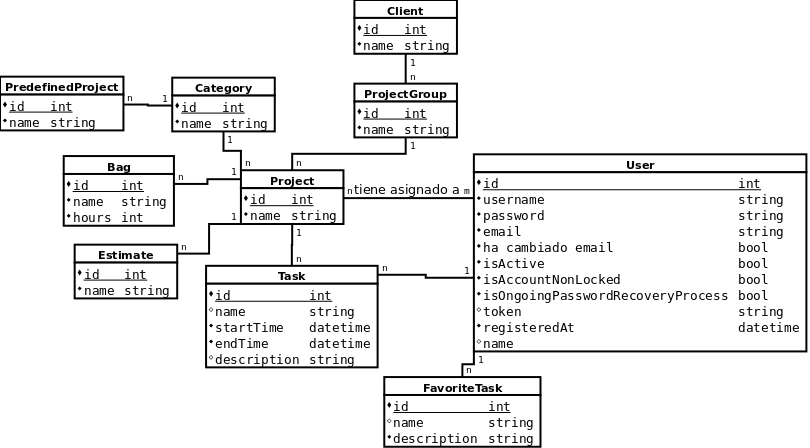
\includegraphics[angle=90,scale=0.6]{img/erDiagram}
    \caption{Diagrama del modelo entidad-relación de la base de
datos\label{fig:erdiag}}
\end{figure}

\subsubsection{Roles}
\label{sec:roles}
Por deseo de los interesados, los usuarios de la aplicación se iban a dividir
en tres grupos principales: gestor con privilegios, gestor, y usuario normal.
En la figura \ref{fig:useCases} se pueden apreciar los diferentes casos de uso
asignados a cada rol. También se puede observar que los roles se heredan, y por
lo tanto el gestor con privilegios heredará los casos de uso del gestor regular
y el usuario regular.

\begin{figure}[p]
    \center
    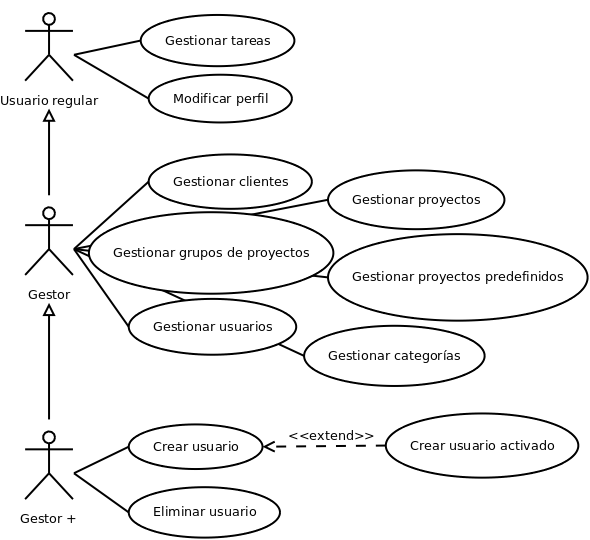
\includegraphics[scale=0.6]{img/useCase}
    \caption{Diagrama de casos de uso de la aplicación}
    \label{fig:useCases}
\end{figure}

\paragraph{Usuario regular}
El usuario con menos privilegios de la aplicación. La idea de este rol es que
los usuarios tengan la sensación de que sólo ellos están utilizando la
aplicación, y por lo tanto, se restringe el acceso a toda la información que no
tenga que ver directamente con él, y por lo tanto puede \textemdash por
gestionar se entiende crear, modificar y eliminar\textemdash:

\begin{itemize}
    \item Consultar su perfil de usuario.
    \item Modificar sus datos de usuario.
    \item Modificar su email y verificarlo.
    \item Modificar su contraseña.
    \item Recuperar la contraseña.
    \item Consultar los proyectos en los que toma parte \textemdash indicándole
        el nombre, grupo del proyecto y la categoría del mismo \textemdash.
    \item Gestionar tareas en los proyectos a los que está asignado.
    \item Gestionar sus tareas favoritas.
\end{itemize}

\paragraph{Gestor}
El gestor es el usuario con privilegios al que se le permite acceder y
modificar casi cualquier apartado de la aplicación. En la siguiente lista
se listan las funcionalidades a las que tiene acceso:

\begin{itemize}
    \item Gestionar clientes.
    \item Gestionar grupos de proyectos y asignarlos a clientes.
    \item Gestionar proyectos y asignarlos a grupos de proyectos, y también
        categorizarlos.
    \item Abrir y cerrar proyectos: de esta forma ningún usuario puede imputar
        más tareas al proyecto.
    \item Gestionar proyectos predefinidos. Además, los proyectos creados a
        partir de un proyecto predefinido verán sus campos modificados si un
        gestor modifica el proyecto predefinido al que está relacionado.
    \item Gestionar categorías.
    \item Gestionar bolsas de horas y asignarlas a proyectos.
    \item Gestionar presupuestos y asignarlos a proyectos.
    \item Gestionar las tareas de cualquier usuario de la aplicación.
    \item Gestionar las tareas favoritas de cualquier usuario de la aplicación.
    \item Modificar el perfil de cualquier usuario de la aplicación.
    \item Activar y desactivar un usuario, lo que permite restringirle por
        completo el acceso a la aplicación.
    \item Asignar y revocar el acceso de los usuarios a los proyectos.
\end{itemize}

\paragraph{Gestor con privilegios}
El gestor con privilegios es el usuario que puede utilizar la aplicación sin
ningún tipo de restricción. Los interesados del proyecto insistieron en que
únicamente un rol específico debería de poder añadir y eliminar usuarios de la
aplicación, ya que opinaban que eso facilitaría la gestión de la misma. Así que
las funcionalidades que se le ofrecen a los usuarios con este rol son:

\begin{itemize}
    \item Crear un usuario en la aplicación.
    \item Eliminar un usuario de la aplicación.
\end{itemize}




  \chapter{Cierre de proyecto y conclusiones}
\section{Seguimiento y control}
\subsection{Alcance}
El alcance especificado ha sido cumplido minuciosamente, y la decisión de haber
separado el proyecto en dos más pequeños parece haber sido un acierto, ya que
me ha permitido desarrollar la aplicación junto con todas sus pruebas
correspondientes, dando como resultado un \glslink{backend}{backend} que podría
ser considerado como estable y sólido.

\subsection{Tiempo}
\label{sec:syc:time}
El proyecto necesitó un total de 484 horas y 25 minutos para completarse, que
se desglosan en 59 horas y 25 minutos de gestión y desarrollo de la
documentación, 385 horas de desarrollo, y 40 horas más para la finalización de
la documentación, retoques finales y preparación de la defensa. La tabla
\ref{table:summary} lo resume.

\begin{table}[h]
\centering
\begin{tabular}{c|c}
\multicolumn{1}{c|}{\textbf{Tarea}} & \textbf{Tiempo invertido} \\ \hline
Gestión & 59 horas y 25 minutos \\ \hline
Desarrollo & 385 horas \\ \hline
Gestión final & 40 horas \\ \hline
\multicolumn{1}{c|}{\textbf{Total}} & 484 horas y 25 minutos
\end{tabular}
\caption{Resumen del tiempo invertido en el proyecto \label{table:summary}}
\end{table}

Esto supera por 34 horas y 25 minutos la cantidad de recursos en forma de
tiempo que se asigna para un \gls{pfm}, y supone aproximadamente una semana
de trabajo más.

\subsubsection{Fase inicial}
Los principales desvíos se han dado en la gestión al inicio del
proyecto. Si bien se estimaba que el inicio del desarrollo comenzaría hacia el
28 de Noviembre de 2017, no es hasta el 14 de Diciembre de 2017 que se tiene
constancia de la primera hora invertida en el desarrollo del producto. Esto se
traduce en 54 horas y 25 minutos, que se invirtieron en las tareas descritas en
la tabla \ref{table:tasks:begin}. También cabe mencionar que durante ese
periodo, la dedicación no fue exclusivamente al proyecto, sino que se compaginó
con otras tareas independientes al mismo, que fueron realizadas para la
empresa. Volviendo a la tabla \ref{table:tasks:begin}, el plasmar toda la
información en el documento \LaTeX llevó más tiempo del deseado, ya que tuve
que volver a aprender a utilizar \LaTeX correctamente, los problemas de
compilación, y sobre todo los problemas de corrección y adecuación de formato.

\begin{table}[h]
\centering
\begin{tabularx}{\textwidth}{X|c}
\multicolumn{1}{c|}{\textbf{Tarea}} & \textbf{Tiempo invertido} \\ \hline
Realizar entrevistas, procesar respuestas y plasmarlas en el documento & 11 horas y 15 minutos \\ \hline
Realizar reuniones con los gestores e interesados de la aplicación & 5 horas \\ \hline
Planificar, diseñar el \glslink{modentrel}{modelo entidad-relación} y la \gls{api} y plasmarlo en el documento & 38 horas y 10 minutos \\ \hline
\multicolumn{1}{c|}{\textbf{Total}} & 54 horas y 25 minutos
\end{tabularx}
\caption{Tareas de la fase inicial \label{table:tasks:begin}}
\end{table}

\subsubsection{Fase de desarrollo}
\paragraph{Diciembre}
\begin{table}[h]
\centering
\begin{tabularx}{\textwidth}{X|c|c}
\multicolumn{1}{c|}{\textbf{Tarea}} & \textbf{Tiempo invertido} & \textbf{Fecha} \\ \hline
& 1h & 14/12/2017 10:00 \textemdash 11:00 \\ \hline
Instalación, configuración y pruebas de Symfony REST & 3 horas y 45 minutos & 21/12/2017 08:45 \textemdash 12:30 \\ \hline
Aprender sobre Symfony HTTP-Foundation & 4 horas & 23/12/2017 09:00 \textemdash 13:00 \\ \hline
Poner en práctica lo aprendido en proyecto de prueba & 4 horas & 23/12/2017 16:00 \textemdash 20:00 \\ \hline
Aprender sobre Symfony Kernel & 4 horas & 25/12/2017 09:00 \textemdash 13:00 \\ \hline
Poner en práctica lo aprendido en proyecto de prueba & 4 horas & 25/12/2017 14:00 \textemdash 18:00 \\ \hline
\multicolumn{1}{c|}{\textbf{Total}} & \multicolumn{2}{c}{20 horas y 45 minutos}
\end{tabularx}
\caption{Tareas de diciembre \label{table:tasks:december}}
\end{table}

Estas tareas se centraron específicamente en la formación y los primeros pasos
con el \glslink{webframework}{framework} Symfony. Al no haber utilizado esta
tecnología para realizar una \gls{api} \gls{rest}, además de que cuando la
utilicé fue hace tiempo, tuve que reciclarme para ponerme al día.

\paragraph{Enero}
\label{sec:tnc:jan}
\textit{Nota: se puede encontrar el informe completo con las tareas detalladas
en el anexo \ref{app:reports:january}}

Uno de mis objetivos con la aplicación era que tuviera una documentación de la
\gls{api} clara y concisa. Es por ello que utilicé la librería
\textit{nelmio/NelmioApiDocBundle}, la cual facilita la documentación de los
diferentes \glslink{endpoint}{endpoints} que conforman una \gls{api}.

En un principio, comencé a usar \textit{FriendsOfSymfony/FOSRestBundle} para
generar los \glslink{endpoint}{endpoints} de la \gls{api}, en vez de utilizar
API Platform. Esto se debe a que en un principio consideré más apropiado utilizar
una librería que no trajera nada por defecto, de forma que me sirviera de formación
para cuando usase el \glslink{webframework}{framework} de API Platform.

Después de esto, me dediqué a configurar el serializador \textemdash véase
\ref{sec:serializer} \textemdash \textit{jms/serializer}, básicamente porque
lo recomendaba la librería \textit{FriendsOfSymfony/FOSRestBundle}.

Una vez configurado, creé el dominio en base al \glslink{modentrel}{modelo 
entidad-relación} que había diseñado, ya que hasta entonces había configurado
el serializador con unas entidades simples, que me permitieran centrarme en
entender cómo trabajar con él sin tener que lidiar con la incertidumbre de
no saber si algo no funciona por causa del serializador o las entidades.

A continuación tocó crear lo que se denominan \textit{fixtures}, o datos de
prueba, con las entidades creadas, de forma que pudiera comprobar que no
existían fallos de diseño en el \glslink{modentrel}{modelo entidad-relación}.
Por desgracia sí que existían problemas no con el diseño, sino con la
implementación del mismo, así que tuve que lidiar con ellos y retocar las
entidades para que funcionaran bien con el \glslink{webframework}{framework}
Symfony.

Con las bases ya controladas, procedí a crear unos \glslink{endpoint}{endpoints}
de prueba con una de las entidades, realicé las pruebas correspondientes y contrasté
los resultados obtenidos. Obviamente hubo mucha prueba y error, pero una vez
conseguido, continué configurando el serializador para intentar limitar la
información que se devolvía dependiendo de los roles establecidos.

Debido a que la fecha de incorporación del alumno que se iba a encargar del \glslink{frontend}{frontend}
de la aplicación estaba muy cerca, me puse manos a la obra con API Platform. La
gran ventaja de este \glslink{webframework}{framework} para \gls{api}s es que
genera automáticamente todos los \glslink{endpoint}{endpoints} a partir de un modelo,
y al tenerlo desarrollado prácticamente me dio la funcionalidad \gls{crud} de toda
la aplicación casi al instante.

Además, las pruebas realizadas hasta el momento con la otra librería me permitieron
integrar una librería de gestión de autentificación \textemdash véase \ref{sec:tech:jwt}
\textemdash y otra de gestión de usuarios \textemdash \textit{friendsofsymfony/user-bundle}
\textemdash.

No obstante, en ese momento uno de los interesados de la aplicación me dijo que no
podía usar una versión de Symfony que no fuera la estable, la cual por aquel
entonces era la versión 3.4. El problema residía en que API Platform usaba una
versión de Symfony superior, y que yo no encontraba la forma de hacer que
los dos \glslink{webframework}{frameworks} fueran compatibles en la versión que
el interesado pedía. Así que mientras encontraba una solución, continué con
el trabajo de formación que había realizado, ya que esto le daba al menos un
\glslink{backend}{backend} funcional al alumno que se había incorporado.

Finalmente encontré dónde surgía la incompatiblidad: cuando intentaba integrar
la versión 3.4 de Symfony con la versión estándar de API Platform, este último
\glslink{webframework}{framework} se quejaba porque la versión de Symfony no
estaba entre sus candidatas para poder funcionar correctamente. Por lo tanto,
indagando en las dependencias de la versión estándar, descubrí que ésta
dependía de otro paquete \textemdash véase \ref{sec:tech:apipack} \textemdash el cual
proveía de toda la funcionalidad necesaria, y aceptaba la versión 3.4 de Symfony
para poder funcionar con ella.

Así que con alivio, pude volver a utilizar API Platform, aunque tuve que
trabajar a marchas forzadas para instalar cuidadosamente, una por una, el resto
de librerías necesarias y asegurándome de que cada paso quedaba bien registrado
en el repositorio donde tenía el código fuente de la aplicación. Al fin y al
cabo, al instalar la versión no estándar de API Platform, había ciertas librerías
que no estaban incluidas \textemdash sobre todo aquellas relativas a las pruebas
o a proporcionar integraciones con otras librerías \textemdash, tenía que repasar
qué es lo que faltaba para incluirlo en la aplicación.

Lo próximo fue meterse de lleno en aprender más sobre API Platform: cómo realizar
los denominados como subrecursos \textemdash véase el párrafo siguiente \textemdash, documentar la API \textemdash ya que a pesar de
que en esencia valía lo que aprendí con mis primeras pruebas de generación de
la documentación, API Platform lo integraba de otra forma \textemdash, configurar
Behat \textemdash véase \ref{sec:tech:behat} \textemdash y solucionar problemas
varios relacionados con la implementación, las pruebas y cumplir con ciertos
requerimientos que ya me empezaba a plantear el otro alumno \textemdash como que
cuando un usuario iniciaba sesión, se mandase también su identificador de usuario
para poder guardarlo y usarlo en peticiones futuras \textemdash.

Sobre los subrecursos: \textit{subresources} en inglés, son aquellos que permiten
obtener unos resultados filtrados con respecto a dos o más entidades. Por ejemplo, si
en un dominio existen las entidades \textit{User} y \textit{Book}, un
subrecurso útil podría ser el de \url{https://example.org/users/21/books} para
obtener la lista de libros del usuario con el identificador 21.

\paragraph{Febrero}
\textit{Nota: se puede encontrar el informe completo con las tareas detalladas
en el anexo \ref{app:reports:february}}
En el modelo algunas de las relaciones se establecieron del tipo \textit{``uno a uno''},
y por algún motivo daban problemas a la hora de insertar datos en la base de datos,
sobre todo con las restricciones de referencia a claves extranjeras en las
operaciones de eliminación. Se invirtió mucho tiempo en investigar qué podría estar
causando este problema, mirando las sentencias \gls{sql} que se generaban e intentando
reproducir paso a paso el error que se estaba produciendo, ya que curiosamente cuando
aplicaba una relación \textit{``uno a uno''} sin el \glslink{webframework}{framework}
API Platform el error no se daba, pero con esa librería en el proyecto sí. Finalmente
tras mucho indagar no pude dar con el problema, y a pesar de haber expuesto
el problema en los canales de soporte pertinentes, nadie parecía encontrar explicación
a lo que ocurría. No obstante el problema se pudo esquivar debido a que después
de analizar el \glslink{modentrel}{modelo entidad-erlación} y debatirlo con los
interesados, se debatió que tenía más sentido sustituir dichas relaciones por unas
del tipo \textit{``uno a n''}, como era en el caso de los presupuestos de un
proyecto, por ejemplo. Aunque la cosa no acabó aquí ya que se dedicó más tiempo a
intentar descubrir qué era lo que causaba el problema, y cómo podría solucionarse,
a pesar de que ya no hiciera falta saberlo, pero no hubo manera. Por lo que finalmente
asumí que probablemente se debería a mi torpeza, y decidí no perder más el tiempo con
ello, a pesar de no quedarme satisfecho.

Continué implementando las pruebas restantes para el resto de entidades de la aplicación,
ya que al estar el segundo alumno desarrollando su parte, no quería entorpecer su avance
y por lo tanto me centraba en implementar las cosas que me iba pidiendo, además de los
requerimientos que tenía que cumplir en la aplicación. Pero siempre con la idea en mente
de completar todas las pruebas, y finalmente pude hacerlo dejando la aplicación en un
estado de \textit{``completamente probada''}. Obviamente estas pruebas evolucionarían
y se modificarían en el futuro, y se añadirían nuevas según desarrollase nuevas cosas,
pero al menos me había quitado esa \textit{espinita}.

Uno de los elementos que supuso un cambio significativo fue la inclusión del
sistema de notificaciones de correo. Se utilizó la librería \textit{swiftmailer/swiftmailer},
debido a que es una librería completísima que facilita el envío de emails utilizando
diferentes protocolos de transporte, soporta cifrado e inicio de sesión en
servidores de correo, permite enviar mensajes en \gls{html}\cite{swiftmailer_symfony} y demás
funcionalidades. También porque es la librería recomendada por el propio \glslink{webframework}{framework}
Symfony, y otras muchas librerías más como por ejemplo la librería de gestión de usuarios
\textit{friendsofsymfony/user-bundle}, la cual utiliza el ya mencionado \textit{Swiftmailer} como
su sistema de gestión de notificaciones de correo electrónico. El problema principal residía en que
a pesar de que API Platform no recomendaba la librería de gestión de usuarios ya mencionada, sí
proveía de un \textit{bridge}\cite{apip_fosuser} o puente que facilitaba la integración en el \glslink{webframework}{framework}
de creación de \gls{api}s. No especificaba cuáles eran los motivos, pero descubrí
uno de ellos al empezar con el desarrollo de las notificaciones de correo: las
funcionalidades de recuperación de contraseña, registro, envío de email de confirmación
y demás requerían de la visita en un recurso web. Por lo tanto, su forma de implementar
las notificaciones, y las generaciones de \gls{url}s con identificadores únicos para
verificar la identidad del usuario que realiza las acciones, estaban muy enfocadas a
proporcionar dichos servicios accediendo a diferentes recursos web. El problema
fundamental residía en que yo estaba desarrollando una \gls{api} \gls{rest}, la
cual debería ser totalmente independiente del \glslink{frontend}{frontend} con el
que se realizan las peticiones, y por lo tanto el hecho de tener que obligar a que
las capas de visualización tuvieran que visitar ciertos recursos web lo consideraba
incoherente y limitante. La solución era tener que realizar \textit{``\glslink{method_overriding}{overrides}''}
de muchísimas partes de la librería de gestión de usuarios, para intentar adaptarla a
mis necesidades. Así que siguiendo el consejo de API Platform, decidí crear un sistema
de usuarios personalizado \textemdash denominado \textit{``custom user provider''} en
el mundo de Symfony\textemdash, justamente porque el trabajo de tener que crear dicho
sistema iba a ser muy similar al de tener que adaptar una librería que no estaba diseñada
para trabajar con \gls{api}s.

Una vez se implementó el sistema de usuarios y se integró con \textit{Swiftmailer},
se pasó a desarrollar un sistema de invitaciones para restringir el registro en la
aplicación: sólo los gestores con privilegios podrían invitar, mediante el envío
automatizado de un correo electrónico desde la aplicación, a ciertos usuarios a ser
parte de la aplicación. Estos usuarios tendrían que validar su correo haciendo clic en
el enlace correspondiente en su correo electrónico, que después el \glslink{frontend}{frontend}
traduciría en una petición a la \gls{api}.

En ése momento, tras revisar el dominio, me di cuenta de que había cometido algunos
errores en el diseño del mismo. No eran errores graves, ya que se podían corregir
fácilmente sin tener que desechar nada de lo desarrollado hasta la fecha, pero requerían
algunos cambios significativos que sobre todo iban a suponer un trabajo considerable
en cuanto a modificar todas las pruebas afectadas. La causa de estos errores se debe a lo siguiente:
antes de realizar el primer \glslink{modentrel}{modelo entidad-relación},
se me presentó un modelo de gestión de la empresa que habían desarrollado y que querían
que sustituyera el modelo de gestión que venían usando hasta entonces. Desarrollé el
\glslink{modentrel}{modelo entidad-relación} equivalente, y lo presenté a los interesados.
No obstante, al validarlo con casos reales y actuales de la empresa, mezclamos conceptos
de la aplicación de gestión que se estaba usando actualmente con los nuevos conceptos del modelo,
y eso unido al \glslink{modentrel}{modelo entidad-relación} diseñado generó muchísima confusión.
A pesar de todo ello, el modelo parecía válido porque no encontramos limitaciones a la hora
de validar los casos reales. Obviamente, y como menciono al principio del párrafo, al revisar
el modelo de nuevo encontré errores que achaqué a la confusión a la hora de debatir este tema,
y mi falta de clarividencia a la hora de plasmar lo que resultó de dichos
debates, aunque en mi defensa he de decir que todos los involucrados en los susodichos debates
salimos algo confundidos de ellos. Aún así, estos errores no suponían cambios muy
significativos, así que adapté el \glslink{modentrel}{modelo entidad-relación} al modelo
final que se presenta en la figura \ref{fig:erdiag}, y presenté los cambios a los interesados,
esta vez sin tanta confusión y con más facilidad debido a las adaptaciones realizadas. Las
consecuencias de estos cambios fueron el tener que adaptar las pruebas de la aplicación y los
correspondientes datos de prueba, lo que supuso un trabajo considerable. Por si eso fuera poco,
el consumo de memoria de las pruebas se disparó, o más bien me fijé que era muy alto. Tras
mucho trastear e investigar por si había realizado algo fuera de lo común que estuviera
malgastando recursos, pregunté en ciertos canales de desarrolladores que me comentaron que
no tenía nada de que preocuparme ya que los consumos estaban dentro de lo normal. De hecho,
de ahí a un tiempo, en una actualización de la librería de pruebas, el consumo descendió muy
significativamente, lo que me dio la prueba definitiva de que realmente ése consumo alto de
recursos no se debía a algún fallo cometido por mi parte.

Tras tenerlo todo atado, continué desarrollando las validaciones de los diferentes campos
de las entidades, ya que hasta este punto únicamente había realizado unas validaciones
genéricas.

Finalmente la última funcionalidad que comencé a implementar en el mes de febrero fue la de la
confirmación del registro por parte de los usuarios, ya que el sistema de invitaciones
de registro funcionaba bien, pero el desarrollo de la confirmación se paró por el asunto
de la modificación del dominio. Esto lo realicé con \gls{dto}s.
Es decir: la validación en el \glslink{webframework}{framework} Symfony se realiza
sobre las entidades \textemdash véase la sección de validaciones \ref{sec:tech:valid}\textemdash,
y por lo tanto estos \textit{DTO}s no son más que pequeñas entidades que sirven para un
propósito específico, como puede ser el recoger el identificador y el correo electrónico
de la confirmación del usuario.

\paragraph{Marzo}
\textit{Nota: se puede encontrar el informe completo con las tareas detalladas
en el anexo \ref{app:reports:march}}

En marzo seguí con las modificaciones en la serialización de las entidades, tanto para
limitar la información que se mostraba a cada rol del usuario como para satisfacer las
necesidades de navegación e información que me pedía el desarrollador del \glslink{frontend}{frontend}.

Después vino una tremenda refactorización de las pruebas de la aplicación. Hasta entonces,
las pruebas consistían en, generalmente, esperar unos valores específicos después de
realizar ciertas peticiones a la base de datos que contenía los datos de prueba. No obstante,
esto suponía un trabajo considerable y repetitivo a la hora de desarrollar una nueva
funcionalidad junto con sus pruebas, o realizar modificaciones a las funcionalidades ya existentes. Por
lo que decidí transformar las pruebas a pruebas de validación con JSON Schema \textemdash véase la sección  \ref{tech:sec:jsonschema} \textemdash
en gran parte, lo que facilitaba mucho la mantenibilidad y reutilización de los esquemas en distintas pruebas.

Finalicé el desarrollo del sistema de verificación de usuarios con el que había comenzado
a trastear a finales de febrero, y aproveché para implementar la funcionalidad de cambio
de contraseña y de cambio de email, todo ello desarrollado y validado con los \gls{dto}s.
Junto con esto, ideé unas pequeñas restricciones
e indicadores que ayudaban a identificar el estado de la cuenta cuando se estaba llevando
a cabo un proceso de cambio de contraseña, recuperación de contraseña o cambio de dirección de correo electrónico: por ejemplo, si se comenzaba
con el proceso de recuperar la contraseña pero el usuario iniciaba sesión antes de completarlo,
se entendía que o bien no lo había solicitado o que ya se había acordado de ella, y por lo tanto
el proceso se daba por finalizado sin que el usuario tuviera que hacer nada más.

Después de limitar la información enviada por cada rol de usuario, terminé de implementar el sistema
de control de acceso, el cual hasta el momento estaba mínimamente desarrollado para probar la restricción de
acceso a ciertos recursos. Terminó siendo muy sencillo gracias a la herencia de roles de Symfony,
que facilita la gestión de los mismos, y que permite hilar muy fino en cuanto a los recursos o
serie de recursos que se quieren restringir mediante el uso de expresiones regulares. Por ejemplo, 
se puede restringir la zona \url{https://example.org/admin} con una expresión regular \textit{\^/admin} que haga que todas las
subrutas como por ejemplo \url{https://example.org/admin/check_status} estén restringidas a un rol.
Los recursos que debían estar disponibles para los tres roles, pero que debían devolver una información u otra,
se restringían programando la lógica de negocio, y aplicando los grupos de serialización
\textemdash véase sección \ref{sec:serializer} \textemdash que se habían desarrollado para las
entidades. Con todo esto, se desarrollaron también las pruebas correspondientes, comprobando que
absolutamente todas las restricciones funcionaban como se pretendía que lo hicieran.

Las últimas funcionalidades que se desarrollaron antes de finalizar con la fase de desarrollo
fueron las de abrir y cerrar proyectos \textemdash restringiendo la posibilidad de añadir o
eliminar tareas por parte de ningún usuario, incluyendo los gestores \textemdash y permitir a
los usuarios que marquen ciertas tareas como favoritas \textemdash para ayudarles a guardar tareas que se
repiten muchas veces y poder reutilizarlas sin tener que volver a introducir todos los datos\textemdash.

El resto del tiempo se dedicó a ajustar la aplicación, arreglar fallos e implementar las
últimas peticiones del otro alumno para flexibilizar el \glslink{backend}{backend}.


\subsection{Calidad}
Se ha alcanzado la calidad mínima especificada en sección de la gestión de
calidad \ref{sec:qua:manag}. En cambio, los elementos de la calidad añadida
no han sido desarrollados, ya que no se ha dispuesto de los recursos suficientes
como para dedicarles un tiempo de desarrollo que fuera a culminar en una
nueva funcionalidad completamente probada. Si no hubiera tenido los desvíos indicados en
la sección de seguimiento y control del tiempo \textemdash véase sección 
\ref{sec:syc:time} \textemdash, creo que la única funcionalidad que pudiera
haber implementado es la onceava.

Finalmente no he podido utilizar la metodología \gls{tdd} en el desarrollo, ya que
generalmente mi intención era poder \textit{publicar} las funcionalidades cuanto
antes para que el otro alumno las tuviera listas para trabajar sobre ellas. Antes de
subir los cambios al repositorio que contenía el código de la aplicación, a veces solía
dejar el código de los cambios en un servidor de pruebas que usábamos para juntar los
dos desarrollos, y de mientras iba realizando las pruebas oportunas para que una vez
se hubiera probado que todo funcionaba bien, subir los cambios al repositorio. Esta
forma de trabajar me permitía tener un colchón de ventaja sobre el otro alumno y por lo
tanto podía trabajar más relajadamente. Por contra, la desventaja
de esta forma de trabajo era que si el otro alumno se ponía a desarrollar sobre una
funcionalidad que no estaba probada, podía ocurrir que después tuviera que cambiar
ligeramente su implementación para adaptarla a las correcciones aplicadas después
de realizar las pruebas, algo que sucedió en alguna ocasión.

\subsection{Riesgos}
Debido a que los riesgos identificados \ref{section:risks} no se han mostrado
significativamente a lo largo del desarrollo del proyecto, no se han tenido que
poner en marcha los planes de contingenciPor contra, la desventaja
de esta forma de trabajo era que si el otro alumno a \ref{section:continplans}.

Es cierto que hubo un momento en el que quizás podría considerarse que el riesgo
de 
\textit{``No tener un producto mínimo que sea funcional cuando el otro
integrante comience a desarrollar su parte.''} estuvo cerca de cumplirse, ya
que tal y como relato en la sección de seguimiento y control de tiempo, la
que corresponde al mes de enero \ref{sec:tnc:jan}, la semana en la que se
incorporó el otro alumno estaba todavía trasteando con las tecnologías de
formación y las del desarrollo del producto final. Aunque también he de decir
que el otro alumno siempre tuvo un \glslink{backend}{backend} operativo con
el que comenzar su desarrollo.

\section{Conclusiones}
Con respecto al producto, se ha logrado el objetivo de construir una \gls{api}
sobre un \glslink{backend}{backend} Symfony que permita ser consumida por
diferentes \glslink{frontend}{frontends}. La aplicación en sí podría resumirse
como un conjunto de librerías cohesionadas con las que se ha desarrollado
un código que realiza la tarea propuesta. Una de las funcionalidades que
quisiera destacar es que la aplicación en sí ha sido construida enteramente con
proyectos de \glslink{opensource}{código abierto}, y es por ello que me apena el no haber conseguido
convencer a los interesados para que el código de la aplicación terminara haciéndose
público bajo una licencia de software libre o código abierto, aunque entiendo perfectamente
los intereses corporativos.

La gestión del proyecto, en mi opinión, ha sido aceptable. Creo que tomé una buena
decisión en no invertir demasiado tiempo en intentar crear un plan de ruta, ya que
después de todo el proceso de desarrollo, no creo que me hubiera acercado a las
estimaciones iniciales. Lo que sí que es cierto es que se retrasó demasiado el
comienzo del desarrollo, y también la formación en la tecnología, lo que en caso
contrario podría haberme permitido desarrollar alguna característica más. El objetivo
de realizar un seguimiento y control exhaustivo se ha cumplido, ya que he tomado nota
de todo lo que he realizado a lo largo del desarrollo, aunque creo que para una
próxima vez sería mejor categorizar las tareas realizadas, ya que de esta forma
se podría elaborar un informe un poco más abstracto, que diera una mejor idea de
todo lo realizado sin tener que leer una por una todas la tareas que se llevaron a cabo.

En cuanto a los objetivos personales, estoy muy satisfecho de haber podido
trabajar en un proyecto con el \gls{webframework}{framework} Symfony, ya que uno
de mis objetivos era poder profundizar y entenderlo mucho mejor, y lo he conseguido.
También quería seguir las mejores prácticas posibles, y es por ello que entre otras
cosas he dedicado mucho tiempo a realizar las pruebas de las funcionalidades
implementadas, y a intentar seguir minuciosamente los patrones y estilos de código
recomendados, para que si en un futuro se abre el código fuente de la aplicación al público
no sólo no se pueda poner en evidencia a la empresa por no seguir las prácticas recomendadas,
sino que tampoco se me pueda poner en evidencia a mi por realizar un desarrollo chapucero. Sé
que esto último es muy subjetivo, y que a pesar de mis buenas intenciones puede que
no haya logrado mi objetivo, pero me quedo muy
tranquilo al saber que he hecho todo lo posible por crear un producto de calidad y
siguiendo lo que muchos expertos recomiendan y publican en las documentaciones
oficiales, blogs y salas de soporte de las diferentes tecnologías.

En general, creo que tanto los interesados como yo hemos terminado muy satisfechos
con el trabajo que este proyecto ha supuesto.


  \appendix


  \chapter{Acrónimos}

\printglossary[type=\acronymtype]

\chapter{Glosario}

\printglossary


  \chapter{Lorem ipsum}

\lipsum[1]


  \chapter{Bibliografía}

\nocite{*}
\printbibliography


\end{document}
